\documentclass[
	a4paper,
	oneside,
	BCOR = 10mm,
	DIV = 12,
	12pt,
	headings = normal,
]{scrartcl}

%%% Length calculations
\usepackage{calc}
%%%

%%% Support for color
\usepackage{xcolor}
\definecolor{lightblue}{HTML}{03A9F4}
\definecolor{red}{HTML}{F44336}
%%%

%%% Including graphics
\usepackage{graphicx}
%%%

%%% Font selection
\usepackage{fontspec}

\setromanfont{STIX Two Text}[
	SmallCapsFeatures = {LetterSpace = 8},
]

\setsansfont{IBM Plex Sans}[
	Scale = MatchUppercase,
]

\setmonofont{IBM Plex Mono}[
	Scale = MatchUppercase,
]
%%%

%%% Math typesetting
\usepackage{amsmath}

\usepackage{unicode-math}
\setmathfont{STIX Two Math}

\usepackage{IEEEtrantools}
%%%

%%% List settings
\usepackage{enumitem}
\setlist[enumerate]{
	label*      = {\arabic*.},
	left        = \parindent,
	topsep      = 0\baselineskip,
	parsep      = 0\baselineskip,
	noitemsep, % override itemsep
}
% List settings for levels 2–4
\setlist[enumerate, 2, 3, 4]{
	label*      = {\arabic*.},
	left        = 0em,
	topsep      = 0\baselineskip,
	parsep      = 0\baselineskip,
	noitemsep, % override itemsep
}

\setlist[itemize]{
	label*      = {—},
	left        = \parindent,
	topsep      = 0\baselineskip,
	parsep      = 0\baselineskip,
	itemsep     = 1\baselineskip,
	noitemsep, % override itemsep
}

\setlist[description]{
	font        = {\rmfamily\upshape\bfseries},
	topsep      = 1\baselineskip,
	parsep      = 0\baselineskip,
	itemsep     = 0\baselineskip,
}

%%%

%%% Structural elements typesetting
\setkomafont{pagenumber}{\rmfamily\upshape}
\setkomafont{disposition}{\rmfamily\bfseries}

% Sectioning
\RedeclareSectionCommand[
	beforeskip = -1\baselineskip,
	afterskip  = 1\baselineskip,
	font       = {\normalsize\bfseries\scshape},
]{section}

\RedeclareSectionCommand[
	beforeskip = -1\baselineskip,
	afterskip  = 1\baselineskip,
	font       = {\normalsize\bfseries\itshape},
]{subsection}

\RedeclareSectionCommand[
	beforeskip = -1\baselineskip,
	afterskip  = 1\baselineskip,
	font       = {\normalsize\bfseries},
]{subsubsection}

\RedeclareSectionCommand[
	beforeskip = -1\baselineskip,
	afterskip  = -0.5em,
	font       = {\normalsize\mdseries\scshape\addfontfeatures{Letters = {UppercaseSmallCaps}}},
]{paragraph}
%%%

%%% Typographic enhancements
\usepackage{microtype}
%%%

%%% Language-specific settings
\usepackage{polyglossia}
\setmainlanguage{ukrainian}
\setotherlanguages{english}
%%%

%%% Captions
\usepackage{caption}
\usepackage{subcaption}

%\DeclareCaptionLabelFormat{closing}{#2)}
%\captionsetup[subtable]{labelformat = closing}

%\captionsetup[subfigure]{labelformat = closing}

\captionsetup[table]{
	aboveskip = 0\baselineskip,
	belowskip = 0\baselineskip,
}

\captionsetup[figure]{
	aboveskip = 1\baselineskip,
	belowskip = 0\baselineskip,
}

\captionsetup[subfigure]{
	labelformat = simple,
	labelformat = brace,
	justification = RaggedRight,
	singlelinecheck = false,
}
%%%

%%% Hyphenated ragged typesetting
\usepackage{ragged2e}
%%%

%%% Table typesetting
\usepackage{booktabs}
\usepackage{longtable}

\usepackage{multirow}

\usepackage{array}
\newcolumntype{v}[1]{>{\RaggedRight\arraybackslash\hspace{0pt}}p{#1}}
\newcolumntype{b}[1]{>{\Centering\arraybackslash\hspace{0pt}}p{#1}}
\newcolumntype{n}[1]{>{\RaggedLeft\arraybackslash\hspace{0pt}}p{#1}}
%%%

%%% Drawing
\usepackage{tikz}
\usepackage{tikzscale}
\usetikzlibrary{positioning}
\usetikzlibrary{arrows.meta} % Stealth arrow tips
%%%

%%% SI units typesetting
\usepackage{siunitx}
\sisetup{
	output-decimal-marker = {,},
	exponent-product      = {\cdot},
	inter-unit-product    = \ensuremath{{} \cdot {}},
	per-mode              = symbol,
}
%%%

% Code Highlighting
\usepackage{minted}
\setmintedinline{
	style = bw,
	breaklines,
}

\newminted[bashterm]{text}{%
	autogobble,%
	breaklines,%
	style=bw,%
}

\newminted[codegeneric]{text}{%
	autogobble,%
	style=bw,%
	breaklines,%
	fontsize=\small,%
}

\newmintinline{bash}{%
}

\newmintinline[minttext]{text}{%
	breaklines,%
	breakanywhere,%
}

%%% Framing code listings
\usepackage{tcolorbox}
\tcbuselibrary{breakable}
\tcbuselibrary{minted}
\tcbuselibrary{skins}

% Text file listing
\newtcblisting[
	auto counter,
	list inside,
	number within = section,
]{listingplaintext}[3][]{%
	minted language = text,
	minted style    = bw,
	minted options  = {
		autogobble,
		linenos,
		tabsize = 4,
		breaklines,
		breakanywhere,
		fontsize = \footnotesize,
	},
	empty,
	sharp corners,
	coltitle = black,
	borderline horizontal = {1pt}{0pt}{black},
	titlerule = {0.5pt},
	titlerule style = {
		black,
	},
	toptitle = 0.3em,
	bottomtitle = 0.3em,
	before skip      = \intextsep,
	after  skip      = \intextsep,
	title            = {Лістинг \thetcbcounter: #2},
	list entry       = {\protect\numberline{\thetcbcounter}#2},
	left = 0em,
	right = 0em,
	%
	listing only,
	breakable,
	%
	label = {#3},%
}

\newtcbinputlisting[
	use counter from = listingplaintext,
	list inside,
	number within = section
]{\inputplaintext}[4][]{%
	minted language = text,
	minted style    = bw,
	minted options  = {
		autogobble,
		linenos,
		tabsize = 4,
		breaklines,
		breakanywhere,
		fontsize = \footnotesize,
	},
	empty,
	sharp corners,
	coltitle = black,
	borderline horizontal = {1pt}{0pt}{black},
	titlerule = {0.5pt},
	titlerule style = {
		black,
	},
	toptitle = 0.3em,
	bottomtitle = 0.3em,
	before skip      = \intextsep,
	after  skip      = \intextsep,
	title            = {Лістинг \thetcbcounter: #3},
	list entry       = {\protect\numberline{\thetcbcounter}#3},
	left = 0em,
	right = 0em,
	%
	listing file={#2},
	listing only,
	breakable,
	%
	label = {#4}
}

\newtcblisting[
	use counter from = listingplaintext,
	list inside,
	number within = section,
]{listingpython}[3][]{%
	minted language = python,
	minted style    = bw,
	minted options  = {
		autogobble,
		linenos,
		tabsize = 4,
		breaklines,
		breakanywhere,
		fontsize = \footnotesize,
	},
	empty,
	sharp corners,
	coltitle = black,
	borderline horizontal = {1pt}{0pt}{black},
	titlerule = {0.5pt},
	titlerule style = {
		black,
	},
	toptitle = 0.3em,
	bottomtitle = 0.3em,
	before skip      = \intextsep,
	after  skip      = \intextsep,
	title            = {Лістинг \thetcbcounter: #2},
	list entry       = {\protect\numberline{\thetcbcounter}#2},
	left = 0em,
	right = 0em,
	%
	listing only,
	breakable,
	%
	label = {#3},
	%
	#1%
}

\newtcbinputlisting[
	use counter from = listingplaintext,
	list inside,
	number within = section
]{\inputpython}[4][]{%
	minted language = python,
	minted style    = bw,
	minted options  = {
		autogobble,
		linenos,
		tabsize = 4,
		breaklines,
		breakanywhere,
		fontsize = \footnotesize,
	},
	empty,
	sharp corners,
	coltitle = black,
	borderline horizontal = {1pt}{0pt}{black},
	titlerule = {0.5pt},
	titlerule style = {
		black,
	},
	toptitle = 0.3em,
	bottomtitle = 0.3em,
	before skip      = \intextsep,
	after  skip      = \intextsep,
	title            = {Лістинг \thetcbcounter: #3},
	list entry       = {\protect\numberline{\thetcbcounter}#3},
	left = 0em,
	right = 0em,
	%
	listing file={#2},
	listing only,
	breakable,
	%
	label = {#4}
}

% Linux command-line listing
\newtcblisting{linuxterm}%
{%
	% Syntax highlighing options
	listing only,%
	minted language = bash,%
	minted options={%
		autogobble,%
		linenos%
	},%
	% Presentation options
	empty,%
	%% Margins
	sharp corners,%
	toptitle = 0.0em,%
	bottomtitle = 0.0em,%
	left = 0em,%
	right = 0em,%
	before skip = \intextsep,%
	after skip = \intextsep,%
}

\newtcblisting{linuxtermout}%
{%
	% Syntax highlighing options
	listing only,%
	minted language = text,%
	minted options={%
		autogobble,%
		linenos%
	},%
	% Presentation options
	empty,%
	%% Margins
	sharp corners,%
	toptitle = 0.0em,%
	bottomtitle = 0.0em,%
	left = 0em,%
	right = 0em,%
	before skip = \intextsep,%
	after skip = \intextsep,%
}

% Dockerfile listings
\newtcblisting[
	use counter from = listingplaintext,
	list inside,
	number within = section,
]{listingdocker}[3][]{%
	minted language = dockerfile,
	minted style    = bw,
	minted options  = {
		autogobble,%
		linenos,
		tabsize = 4,
		breaklines,
		breakanywhere,
		fontsize = \footnotesize,
	},
	empty,
	sharp corners,
	coltitle = black,
	borderline horizontal = {1pt}{0pt}{black},
	titlerule = {0.5pt},
	titlerule style = {
		black,
	},
	toptitle = 0.3em,
	bottomtitle = 0.3em,
	before skip      = \intextsep,
	after  skip      = \intextsep,
	title            = {Лістинг \thetcbcounter: #2},
	list entry       = {\protect\numberline{\thetcbcounter}#2},
	left = 0em,
	right = 0em,
	%
	listing only,
	breakable,
	%
	label = {#3},%
}

% Docker Compose listings
\newtcblisting[
	use counter from = listingplaintext,
	list inside,
	number within = section,
]{listingdockercompose}[3][]{%
	minted language = yaml,
	minted style    = bw,
	minted options  = {
		autogobble,%
		linenos,
		tabsize = 4,
		breaklines,
		breakanywhere,
		fontsize = \footnotesize,
	},
	empty,
	sharp corners,
	coltitle = black,
	borderline horizontal = {1pt}{0pt}{black},
	titlerule = {0.5pt},
	titlerule style = {
		black,
	},
	toptitle = 0.3em,
	bottomtitle = 0.3em,
	before skip      = \intextsep,
	after  skip      = \intextsep,
	title            = {Лістинг \thetcbcounter: #2},
	list entry       = {\protect\numberline{\thetcbcounter}#2},
	left = 0em,
	right = 0em,
	%
	listing only,
	breakable,
	%
	label = {#3},%
}


% Customize minted line numbers
\renewcommand{\theFancyVerbLine}{\ttfamily\scriptsize\arabic{FancyVerbLine}}

%%%

%%% Typeset menus and keys
\usepackage{menukeys}[
	os=win,
]
%%%

%%% Links and hyperreferences
\usepackage{hyperref}
\hypersetup{
	bookmarksnumbered = true,
	colorlinks      = false,
	linkbordercolor = red,
	urlbordercolor  = lightblue,
	pdfborderstyle  = {/S/U/W 1.5},
}
%%%

%%% Length adjustment

% Set baselineskip, default is 14.5 pt
\linespread{1.068966} % ~15.5 pt
\setlength{\emergencystretch}{1em}
\setlength{\parindent}{1.5em}
\newlength{\gridunitwidth}
\setlength{\gridunitwidth}{\textwidth / 12}
%%%

%%% Custom commands
\newcommand{\allcaps}[1]{%
	{%
		\addfontfeatures{%
			Letters = UppercaseSmallCaps,
			LetterSpace = 8,%
		}%
		#1%
	}%
}
\newcommand{\filename}[1]{\texttt{#1}}
\newcommand{\progname}[1]{\texttt{#1}}
\newcommand{\commandname}[1]{\texttt{#1}}
\newcommand{\modulename}[1]{\texttt{#1}}
\newcommand{\ifname}[1]{\texttt{#1}} % typesets a network interface's name

\newcommand{\transeng}[1]{{англ.}~\textit{\textenglish{#1}}}
%%%

%%% Custom math commands
\newcommand{\longvar}[1]{\mathit{#1}}
%%%

\begin{document}

\begin{titlepage}
		\begin{center}
			Міністерство освіти і~науки України\\
			Національний авіаційний університет\\
			Факультет кібербезпеки, комп'ютерної та~програмної інженерії\\
			Кафедра комп'ютеризованих систем управління

			\vspace{\fill}
				Лабораторна робота №~2.3\\
				з~дисципліни «Захист інформації в~комп'ютерних системах»\\
				на~тему «Криптографічний захист даних у~файлових системах»

			\vspace{\fill}

			\begin{flushright}
				Виконав:\\
				студент \allcaps{ФККПІ}\\
				групи \allcaps{СП}-425\\
				Клокун В.\,Д.\\
				Перевірила:\\
				Супрун О.\,М.
			\end{flushright}

			Київ 2019
		\end{center}
	\end{titlepage}

	\section{Мета роботи}
		Ознайомитися з~основними проблемами захисту інформації у~файлових системах та~засобами їх~розв’язання.

	\section{Завдання роботи}
		Встановити програмне забезпечення для~криптографічного захисту даних у~файлових системах та~навчитися використовувати його функції.

	\section{Хід~роботи}
		Щоб~виконати завдання лабораторної роботи, встановлюємо та~запускаємо програму~\textenglish{VeraCrypt}. Після запуску бачимо головне меню програми~(рис.~\ref{fig:vc-main-menu})

		\begin{figure}[!htbp]
			\centering
			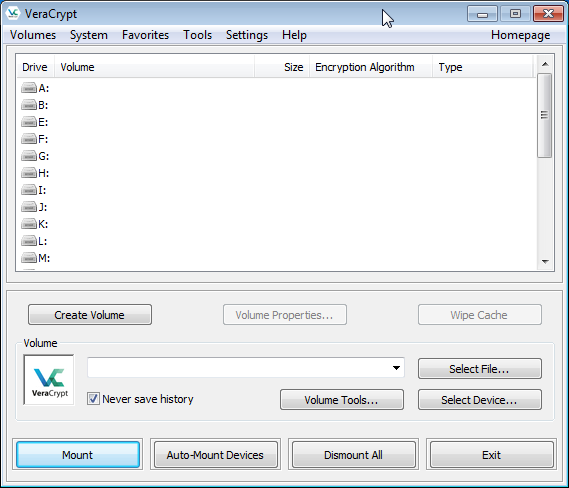
\includegraphics[height = 10 \baselineskip]{./assets/01.png}
			\caption{Головне меню програми~\textenglish{VeraCrypt}}
			\label{fig:vc-main-menu}
		\end{figure}

		Створюємо новий том. Для~цього у~головному меню натискаємо кнопку~«\textenglish{Create Volume}»; з'явиться помічник зі~створення тому~(рис.~\ref{fig:vc-volcr-wizard}). У~помічнику можна обрати, як~створити том: створити зашифрований файл-контейнер, зашифрувати несистемну партицію або~диск чи~зашифрувати системну партицію або~диск. Обираємо створення зашифрованого контейнера і~переходимо далі.

		\begin{figure}[!htbp]
			\centering
			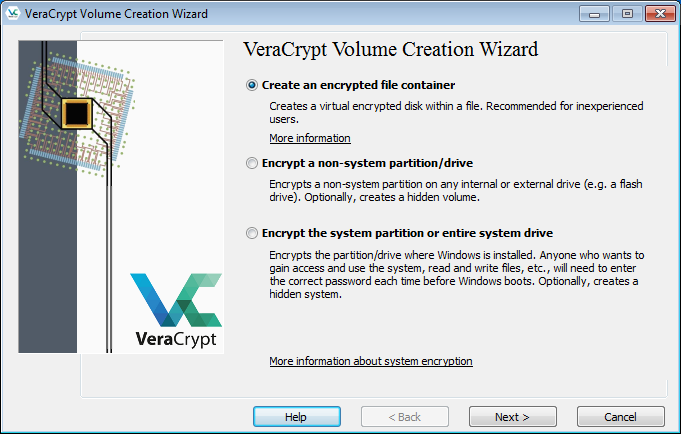
\includegraphics[height = 10 \baselineskip]{./assets/02.png}
			\caption{Помічник зі~створення тому~\textenglish{VeraCrypt}}
			\label{fig:vc-volcr-wizard}
		\end{figure}

		Після переходу далі відкрився екран вибору типу створюваного тому: стандартного або~прихованого~(рис.~\ref{fig:vc-volcr-wizard-vol-type}). Стандартний том~створює звичайний зашифрований контейнер, тоді як~прихований том~— це~ще~один том~\textenglish{VeraCrypt}, який знаходиться всередині стандартного тому~\textenglish{VeraCrypt}.

		\begin{figure}[!htbp]
			\centering
			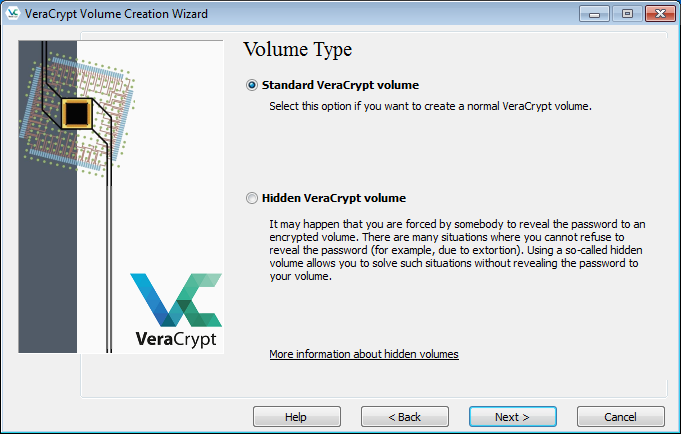
\includegraphics[height = 10 \baselineskip]{./assets/03.png}
			\caption{Вибір типу тому~\textenglish{VeraCrypt}}
			\label{fig:vc-volcr-wizard-vol-type}
		\end{figure}

		Обравши тип~тому, обираємо, де~його зберігати. Для~цього натискаємо кнопку «\textenglish{Select File...}» і~вказуємо розміщення і~ім'я~файлу, в~якому зберігатиметься контейнер~(рис.~\ref{fig:vc-volume-path}).

		\begin{figure}[!htbp]
			\centering
			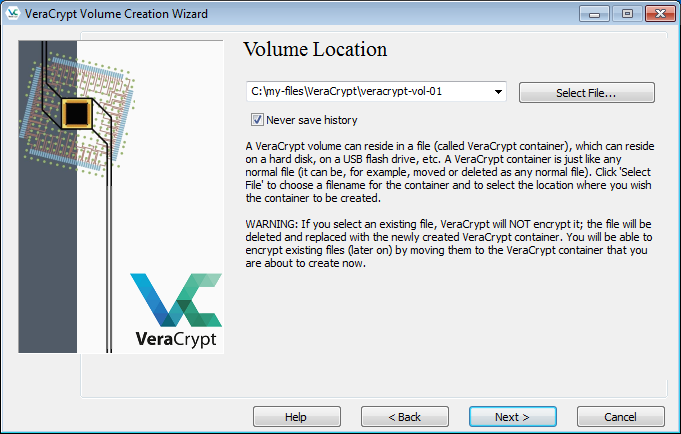
\includegraphics[height = 10 \baselineskip]{./assets/04.png}
			\caption{Вибір розміщення тому~\textenglish{VeraCrypt}}
			\label{fig:vc-volume-path}
		\end{figure}

		Обравши розміщення тому, обираємо параметри шифрування, яке~буде використовуватись у~ньому~(рис.~\ref{fig:vc-enc-settings}). За~замовчуванням встановлені надійні значення, тому більшості користувачів варто залишити їх~якими вони є.

		\begin{figure}[!htbp]
			\centering
			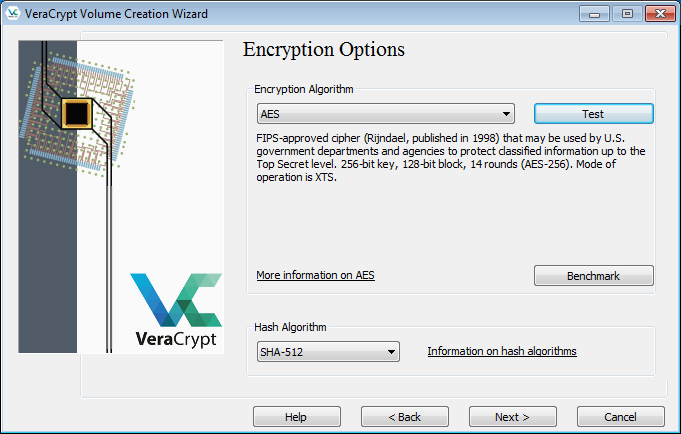
\includegraphics[height = 10 \baselineskip]{./assets/05.png}
			\caption{Вибір налаштувань шифрування тому~\textenglish{VeraCrypt}}
			\label{fig:vc-enc-settings}
		\end{figure}

		Після налаштування параметрів шифрування, необхідно задати розмір тому~(рис.~\ref{fig:vc-vol-size}). Мінімальний розмір залежить від~файлової системи, а~максимальний обмежений лише вільним місцем на~диску.

		\begin{figure}[!htbp]
			\centering
			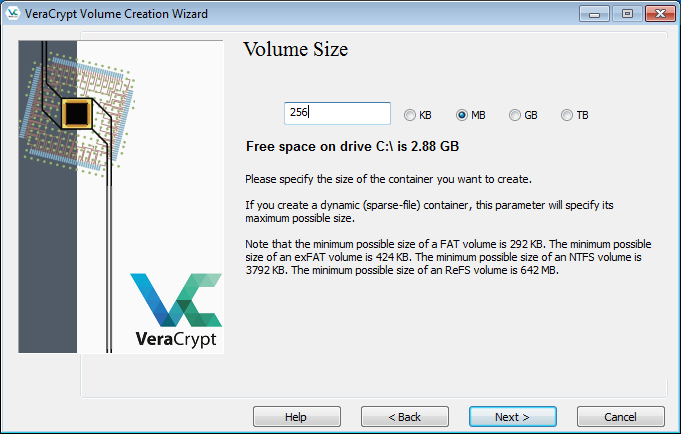
\includegraphics[height = 10 \baselineskip]{./assets/06.png}
			\caption{Установка розміру тому~\textenglish{VeraCrypt}}
			\label{fig:vc-vol-size}
		\end{figure}

		Коли розмір тому встановлений, необхідно задати для~нього пароль~(рис.~\ref{fig:vc-vol-password}). Пароль має~бути надійним, адже від~нього залежить безпека усіх даних, які~зберігаються у~томі.

		\begin{figure}[!htbp]
			\centering
			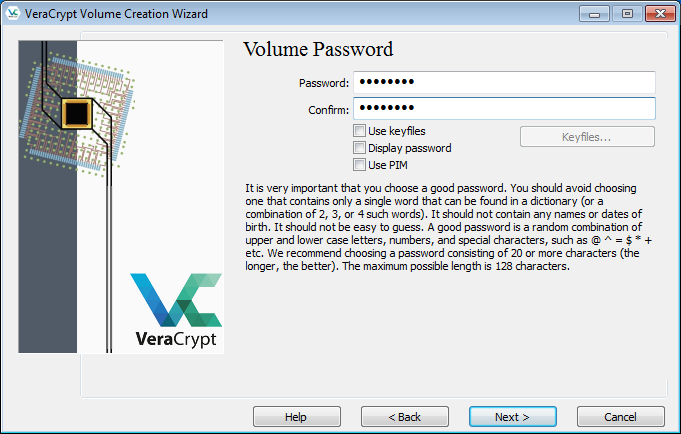
\includegraphics[height = 10 \baselineskip]{./assets/07.png}
			\caption{Установка пароля тому~\textenglish{VeraCrypt}}
			\label{fig:vc-vol-password}
		\end{figure}

		Після установки пароля програмі необхідні випадкові дані. Для~цього вона збирає їх, зчитуючи рух~користувача мишкою~(рис.~\ref{fig:vc-randomness}).

		\begin{figure}[!htbp]
			\centering
			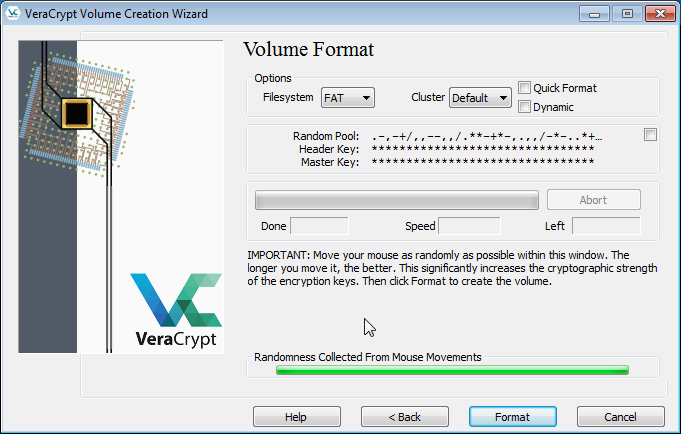
\includegraphics[height = 10 \baselineskip]{./assets/08.png}
			\caption{Збір випадкових даних програмою~\textenglish{VeraCrypt}}
			\label{fig:vc-randomness}
		\end{figure}

		Зібравши необхідну кількість випадкових даних, програма створює контейнер, повідомляє користувача за~допомогою відповідного повідомлення і~переходить до~фінального вікна~(рис.~\ref{fig:vc-wizard-final}).

		\begin{figure}[!htbp]
			\centering
			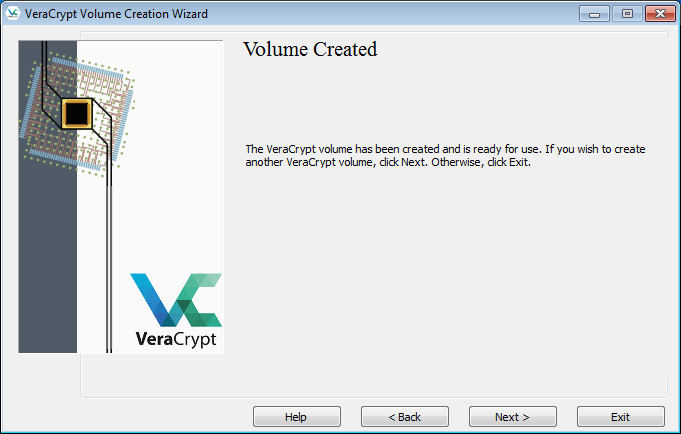
\includegraphics[height = 10 \baselineskip]{./assets/11.png}
			\caption{Фінальне вікно помічника зі~створення зашифрованого контейнера програми~\textenglish{VeraCrypt}}
			\label{fig:vc-wizard-final}
		\end{figure}

		Тепер, коли контейнер створений, можна змонтувати його і~працювати з~його даними. Для~цього відкриваємо головне меню програми~\textenglish{VeraCrypt}, обираємо файл з~контейнером і~натискаємо кнопку~«\textenglish{Mount}»~(рис.\ref{fig:vc-mount}).

		\begin{figure}[!htbp]
			\centering
			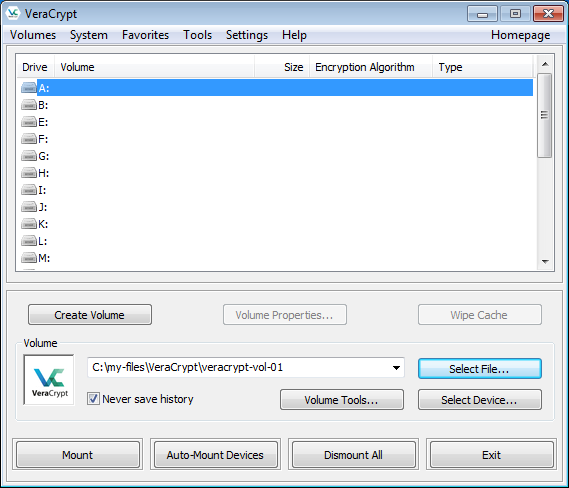
\includegraphics[height = 10 \baselineskip]{./assets/12.png}
			\caption{Вибір зашифрованого контейнера для~монтування}
			\label{fig:vc-mount}
		\end{figure}

		Після натискання на~кнопку з'явиться діалогове вікно, яке~запросить користувача ввести пароль або~підтвердити свою особистість іншим способом, щоб~змонтувати контейнер~(рис.~\ref{fig:vc-password-prompt}).

		\begin{figure}[!htbp]
			\centering
			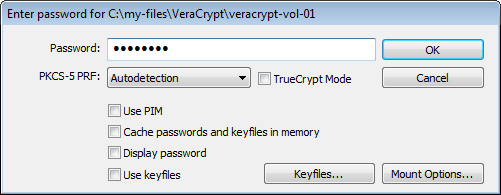
\includegraphics[height = 6 \baselineskip]{./assets/13.png}
			\caption{Діалогове вікно для~монтування контейнера}
			\label{fig:vc-password-prompt}
		\end{figure}

		Зчитавши пароль, програма спробує змонтувати контейнер і~в~разі успіху він~з'явиться у~головному меню навпроти літери, яку~користувач обрав під~час~монтування~(рис.~\ref{subfig:vc-res-vc}). Також, контейнер буде підключений і~доступний з~Провідника~\textenglish{Windows}~(рис.~\ref{subfig:vc-res-explorer}).

		\begin{figure}[!htbp]
			\begin{subfigure}[b]{6\gridunitwidth - 1em / 2}
				\centering
				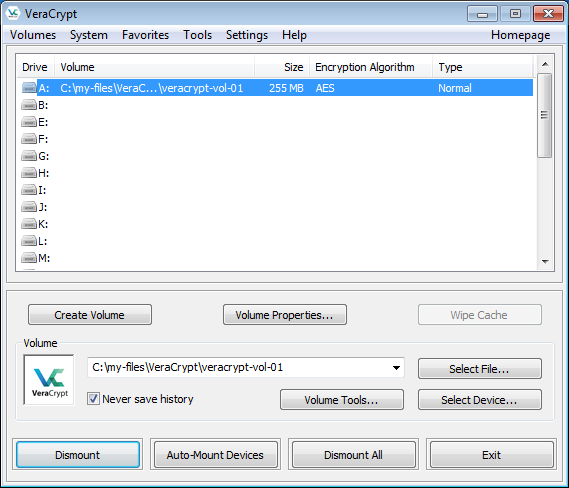
\includegraphics[width = \columnwidth]{./assets/15.png}
				\caption{}
				\label{subfig:vc-res-vc}
			\end{subfigure}%
			\hspace{1em}%
			\begin{subfigure}[b]{6\gridunitwidth - 1em / 2}
				\centering
				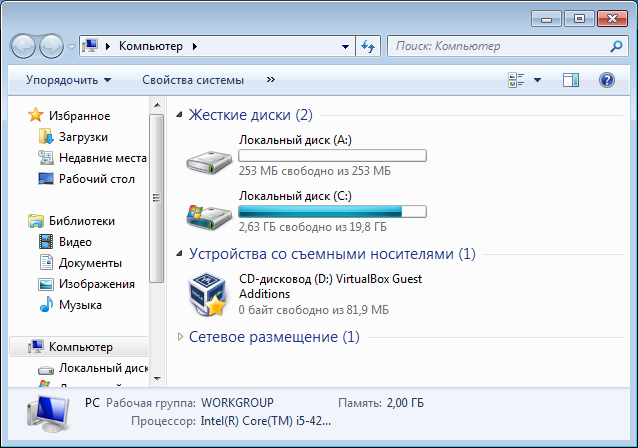
\includegraphics[width = \columnwidth]{./assets/16.png}
				\caption{}
				\label{subfig:vc-res-explorer}
			\end{subfigure}
			\caption{Результат монтування контейнера}
			\label{fig:vc-res}
		\end{figure}

		Отже, тепер контейнер змонтований і~готовий до~роботи з~його файлами.

	\section{Висновок}
		Виконуючи дану лабораторну роботу, ми~ознайомилися з~основними проблемами захисту інформації у~файлових системах та~засобами їх~розв’язання.
\end{document}
